% 2006 上海卷文科 Q19；按固定扫描件印刷页 330 重绘，线型与连接关系为核对重点。
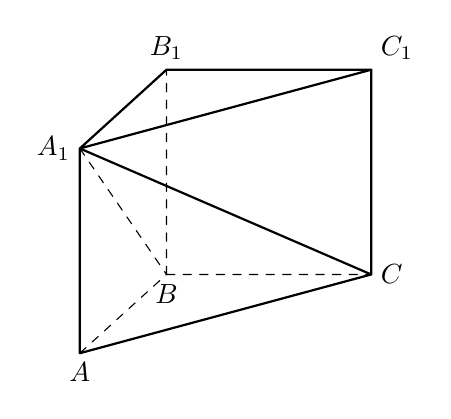
\begin{tikzpicture}[line cap=round,line join=round]
  \coordinate (A)  at (0,0);
  \coordinate (B)  at (1.1,1.0);
  \coordinate (C)  at (3.7,1.0);
  \coordinate (A1) at (0,2.6);
  \coordinate (B1) at (1.1,3.6);
  \coordinate (C1) at (3.7,3.6);

  % 来源图中的隐藏棱以及 A_1B 辅助线为虚线。
  \draw[dashed] (A)--(B) (B)--(C) (B)--(B1) (A1)--(B);
  \draw[thick] (A)--(A1) (C)--(C1) (A)--(C);
  \draw[thick] (A1)--(B1) (B1)--(C1) (A1)--(C1);
  \draw[thick] (A1)--(C);

  \node[below] at (A) {$A$};
  \node[below] at (B) {$B$};
  \node[right] at (C) {$C$};
  \node[left] at (A1) {$A_1$};
  \node[above] at (B1) {$B_1$};
  \node[above right] at (C1) {$C_1$};
\end{tikzpicture}
